\documentclass{../../../fal_assignment}
\graphicspath{ {../../../} }

\usepackage{enumitem}
\setlist{nosep} % Make enumerate / itemize lists more closely spaced
\usepackage[T1]{fontenc} % http://tex.stackexchange.com/a/17858
\usepackage{url}
\usepackage{todonotes}

\title{COMP110 Worksheet 9: TIS-100}
\module{COMP110}
\author{Ed Powley}
\version{3.0}

\begin{document}

\maketitle

\section*{Introduction}

\begin{marginquote}
``The Tesselated Intelligence System is a massively parallel computer architecture comprised of non-uniformly
interconnected heterogeneous nodes. The Tessellated Intelligence System is ideal for applications requiring complex
data stream processing, such as automated financial trading, bulk data collection, and civilian behavioural analysis.''

--- TIS-100 Reference Manual
\end{marginquote}
\marginpicture{flavour_pic}{
    \emph{TIS-100} is a puzzle game in which players must write assembly code to process data streams
    in increasingly complex ways.
}

\textbf{TIS-100} is a puzzle game released in 2015 by independent developers Zachtronics.
The gameplay consists of writing assembly code for a fictional parallel computer architecture,
and as such requires skills in low-level programming.

To complete this worksheet:
\begin{enumerate}[label=(\alph*)]
	\item \textbf{Play} TIS-100 --- it is available on the PCs in the Games Academy, or can be purchased from Steam for around \textsterling 5;
 	\item \textbf{Complete} the first thirteen levels of the game, upto and including ``Signal Multiplier'';
 	\item \textbf{Complete} the optional stretch goals.
\end{enumerate}

\section*{Submission instructions}

Begin by \textbf{forking} the GitHub repository at the following URL:

\url{https://github.com/Falmouth-Games-Academy/comp110-worksheet-9}

Play TIS-100.
Once you are ready to upload your work, click the ``Open Save Directory'' button within the game (on the level select screen),
navigate up one directory, and commit and push the contents of this directory to your GitHub repository.
The contents of your repository should look like the following --- noting the \texttt{save.dat} file in the root,
and the \texttt{save} directory containing your actual solutions:

\begin{center}
	\fbox{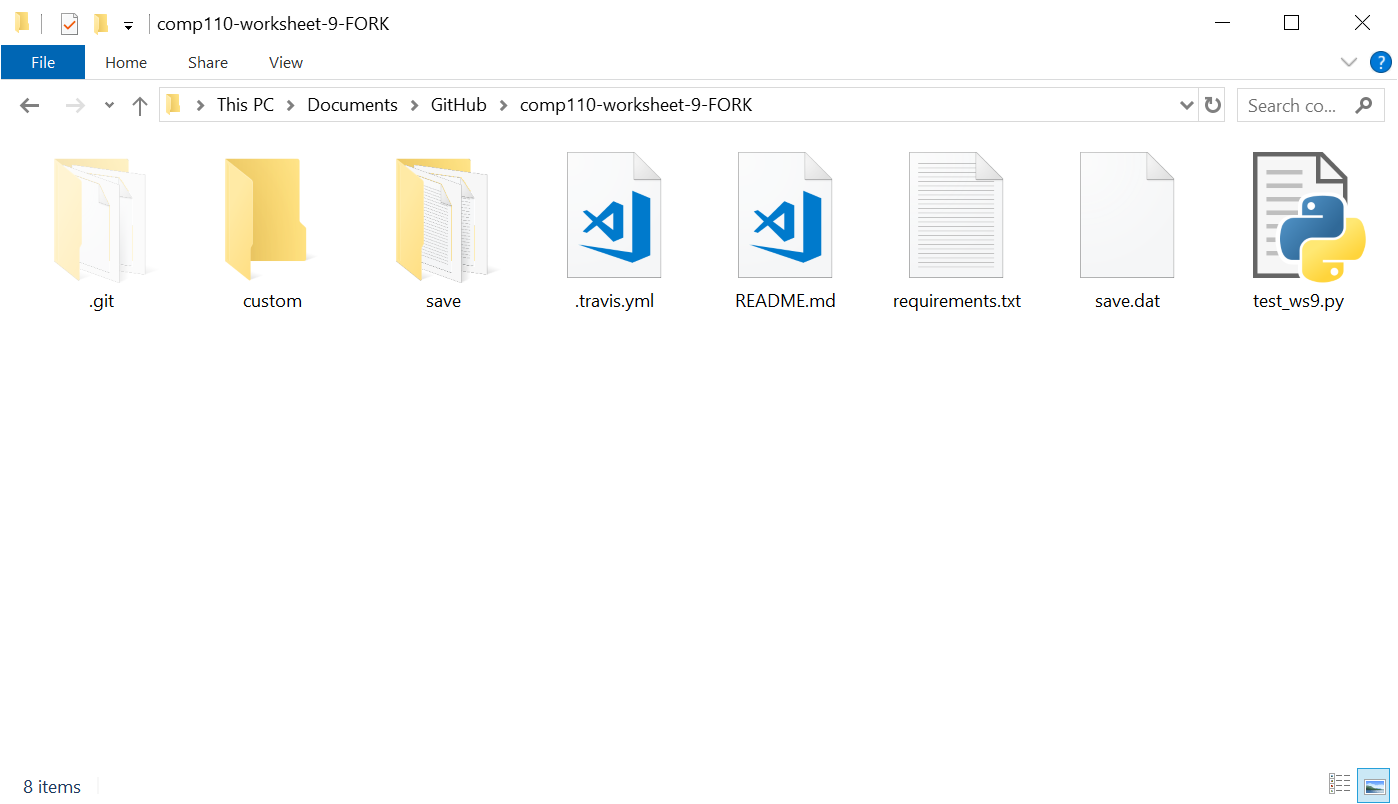
\includegraphics[width=\textwidth]{folder}}
\end{center}

\section*{Stretch goals}

The basic task for this worksheet is to complete the first 13 non-sandbox levels of the game, upto and including ``Signal Multiplier''.
Partial credit will be awarded for completing some portion of these levels --- if you are stuck on a particular level, skip it and carry on to solve the rest.

Extra marks are available for completing one or more of the following stretch goals:

	\begin{itemize}
		\item Solve ``Differential Converter'' in 250 cycles or fewer;
		\item Solve ``Sequence Counter'' in 4 nodes or fewer;
		\item Continue progressing through the game to unlock the bottom row of the level select screen, and solve ``Sequence Sorter''. (I was stuck on this level for several weeks when I first played TIS-100!)
	\end{itemize}

\begin{markingrubric}
	\firstcriterion{Basic competency threshold}{30\%}
		\grade\fail	A reasonable attempt at the worksheet was not submitted by the formative deadline.
	\gradespan{5}{A reasonable attempt at the worksheet was submitted by the formative deadline.
		\par		There is no evidence of academic misconduct.}
		
    \criterion{PROCESS: Task completion}{70\%}
        \grade\fail No tasks have been completed.
        \grade At least one level has been completed.
        \grade The first 13 levels have been completed.
        \grade The first 13 levels have been completed.
            \par One of the stretch goals listed above has been completed.
        \grade The first 13 levels have been completed.
            \par Two of the stretch goals listed above has been completed.
        \grade The first 13 levels have been completed.
            \par All three of the stretch goals listed above has been completed.
\end{markingrubric}

\end{document}
